\section{Persistence modules}

This section serves to build a single algebraic structure called a \emph{persistence module}, for which we can describe the concept of \emph{persistence}, but to do so we require tools from \emph{category theory} and \emph{module theory}. We also touch on cohomology, as it is needed for a speed-up in the persistent homology algorithm. 

We move to form a bijection between the isomorphism classes of \emph{persistence modules} of finite type over a field and the finite sets of $\mathcal P$-intervals.

\subsection{A brief touch on category theory}

Category theory has the ambitious goal to generalize all of mathematics in terms of \emph{categories}, irrespective of the underlying structure of such objects.

\begin{definition}[Category]
    A \emph{category} $C$ consists of
    \begin{enumerate}
        \item a class $\ob(C)$ of \emph{objects};
        \item a class $\hom(C)$ of \emph{morphisms} between objects;
        \item a \emph{domain} class function $\dom: \hom(C) \to \ob(C)$;
        \item a \emph{codomain} class function $\cod: \hom(C) \to \ob(C)$; and
        \item for every $f,g \in \hom(C)$ such that $\cod(f) = \dom(g)$, a morphism denoted $g \circ f$ (or $gf$) called their \emph{composite}
    \end{enumerate}
    such that for all $f, g, h \in \hom(C)$ and $x, y \in \ob(C)$,
    \begin{enumerate}
        \item if $\cod(f) = \dom(g)$, then $\dom(g \circ f) = \dom(f)$ and $\cod(g \circ f) = \cod(g)$;
        \item there exists a morphism $\id_x \in \hom(C)$ (called the \emph{identity morphism}) such that $\dom(\id_x) = x$ and $\cod(\id_x) = x$;
        \item if $\cod(f) = \dom(g)$ and $\cod(g) = \dom(h)$, then $(h \circ g) \circ f = h \circ (g \circ f)$; and
        \item if $\dom(f) = x$ and $\cod(f) = y$, then $\id_y \circ f = f \circ \id_x$.
    \end{enumerate}
\end{definition}

Note here that there is little in the way of description of what is meant by an \emph{object} and a \emph{morphisms}, which is the purpose at this level of abstraction.

\begin{example} \hspace{0em}
    \begin{enumerate}
        \item The category of \emph{sets and functions}, denoted as $\Set$, is a valid category.
        \item The category of \emph{abelian groups and group homomorphisms}, denoted $\Ab$, is another valid category. It is a \emph{subcategory} of the category of \emph{groups and group homomorphisms}, denoted $\Grp$.
    \end{enumerate}
\end{example}

\begin{definition}[Isomorphism]
    Let $C$ be a category and $x,y \in \ob(C)$. A morphism $f: \hom(x, y)$ is an \emph{isomorphism} if there exists a morphism $f^{-1} \in \hom(y, x)$ such that $f \circ f^{-1} = \id_y$ and $f^{-1} \circ f = \id_x$. We call $f^{-1}$ the \emph{inverse} of $f$.
\end{definition}

This gives us a generalisation of isomorphisms as we know them for groups, graphs, vector spaces, topology, etc.

We now define a mapping \emph{between} categories. For a category $C$ and $x,y \in \ob(C)$, $\hom(x, y)$ denotes a subclass of of $\hom(C)$ such that, if $f \in \hom(x,y)$, then $\dom(f) = x$ and $\cod(f) = y$. Denote such a morphism by $f: x \to y$.

\begin{definition}[Functor]
    Let $C$ and $D$ be categories. A \emph{functor} $F: C \to D$ from $C$ to $D$ is a mapping that
    \begin{enumerate}
        \item associates each $x \in \ob(C)$ to a $F(x) \in \ob(D)$;
        \item associates each $f \in \hom(C)$ to a $F(f) \in \hom(D)$ such that
              \begin{enumerate}
                  \item $\dom(F(f)) = F(\dom(f))$ and $\cod(F(f)) = F(\cod(f))$;
                  \item for every $x \in \ob(C)$, we have $F(\id_x) = \id_{F(x)}$; and
                  \item for all morphism $f, g \in \hom(C)$ such that $\cod(f) = \dom(g)$, we have $F(g \circ f) = F(g) \circ F(f)$.
              \end{enumerate}
    \end{enumerate}
\end{definition}

Functors between categories must preserve identity morphisms and composition of morphisms.

\begin{example}[Examples of functors] \hspace{0em}
    \begin{enumerate}
        \item For any category $C$, we may define the \emph{identity endofunctor} (an endofunctor is functor that maps from a category to itself) that maps all objects to itself and all morphisms to itself, we denote this functor $\id_C$.
        \item We may define \emph{homology} as a \emph{contravariant} functor from the category of chain complexes to the category of abelian groups (or modules, which we will later see). A contravariant functor is defined in the same way as a regular functor, except for the fact that they \emph{reverse composition} and switches the domain and codomain; that is $F(g \circ f) = F(f) \circ F(g)$ (in (ii)(b) above) and if $f: x \to y$, then $F(f): F(y) \to F(x)$.
        \item Another interesting example (which we do not go into details here) is the abelianization functor mapping from the category of groups to the category of abelian groups. The abelianization of some group $G$ is the quotient of $G$ by the relation $xy = yx$ for all $x,y \in G$, and the construction of this functor is as one would expect (using the canonical quotient map).
    \end{enumerate}
\end{example}

\begin{proposition} \label{lem:functors-perserve-isomorphisms}
    Functors preserve isomorphisms.
\end{proposition}

\begin{proof}
    Let $C$ and $D$ be categories and $F: C \to D$ a functor. Let $f \in \hom(C)$ be an isomorphism with inverse $f^{-1}$. Then
    \[F(f) \circ F(f^{-1}) = F(f \circ f^{-1}) = F(\id_y) = \id_{F(y)}\]
    and
    \[F(f^{-1}) \circ F(f) = F(f^{-1} \circ f) = F(\id_x) = \id_{F(x)},\]
    thus $F(f) \in \hom(D)$ is an isomorphism.
\end{proof}

\begin{definition}[Natural isomorphism]
    Let $F$ and $G$ be functors between categories $C$ and $D$. A \emph{natural transformation} $\eta = \{\eta_x\}_{x \in C}$ from $F$ to $G$ is a family of morphisms such that $\eta_x: F(x) \to G(x)$ and the following diagram commutes for all $f: x \to y$ in $C$.
    \begin{center}
        % https://tikzcd.yichuanshen.de/#N4Igdg9gJgpgziAXAbVABwnAlgFyxMJZABgBpiBdUkANwEMAbAVxiRADEAKADwEoQAvqXSZc+QijIBGKrUYs2AcR78hI7HgJEATKRnV6zVohDKAnquEgMG8TvKzDCk+dWyYUAObwioAGYAThAAtkhkIDgQSFIG8sYgADoJMDh0APrcINQMdABGMAwACqKaEiABWJ4AFjiCVoEhSADM1JFIunJGbEkp6WZ1-kGhiOFtiC2dzhycfpaDjYgxEVGIHU7xyrNZIDn5RSV2JhXVtQIUAkA
        \begin{tikzcd}
            F(x) \arrow[d, "\eta_x"'] \arrow[rr, "F(f)"] &  & G(y) \arrow[d, "\eta_y"] \\
            G(x) \arrow[rr, "G(f)"']                     &  & G(y)
        \end{tikzcd}
    \end{center}
    If $\eta_x$ is an isomorphism for every $x \in \ob(C)$, then $\eta$ is said to be a \emph{natural isomorphism}. If such an $\eta$ exists, $F$ and $G$ are said to be naturally isomorphic, denoted $F \simeq G$.
\end{definition}

\begin{definition}[Equivalence of categories]
    Let $C$ and $D$ be categories. An \emph{equivalence} of two categories is a pair of functors $F: C \to D$ and $G: D \to C$ alongside two natural isomorphisms $F \circ G \simeq \id_D$ and $G \circ F \simeq \id_C$.
\end{definition}

If such an equivalence of categories exists between categories $C$ and $D$, then $C$ and $D$ are said to be \emph{equivalent}, denoted $C \simeq D$, and in the definition above $F: C \to D$ (or $G: D \to C$) are said to define an equivalence of categories. Equivalence of categories is more analogous to \emph{homotopy equivalence} from homotopy theory then it is to homeomorphic; however, this is not a perfect analogy.

Equivalence of categories do not present particularly strong correspondence between objects within each category; however, it does provide a bijection between the isomorphisms within each category.

\begin{corollary} \label{cor:equivalence-functor-give-bijection-on-isomorphisms}
    Let $F$ be a functor which defines an equivalence between categories $C$ and $D$. Then $f \in \hom(C)$ is an isomorphism if and only if $F(f) \in \hom(D)$ is an isomorphism.
\end{corollary}

\subsection{On modules and their structure}

Here we briefly touch on \emph{module theory} and a fundamental result from abstract algebra on the structure of finitely generated modules over principal ideal domain.

A module is a generalization of a vector spaces, but we replace the field of scalars with a ring.

\begin{definition}[Module] \label{def:module}
    Let $R$ be a commutative ring with multiplicative identity $1$. A \emph{$R$-module} $M$ consists of an abelian group $(M, +)$ and an operation $\cdot: R \times M \to M$ such that for all $r, s \in R$ and $m, n \in M$, we have
    \begin{enumerate}
        \item $(r + s) \cdot m = r \cdot m + s \cdot m$;
        \item $(rs) \cdot m = r \cdot (s \cdot m)$;
        \item $r \cdot (m + n) = r \cdot m + r \cdot n$; and
        \item $1 \cdot m = m$.
    \end{enumerate}
\end{definition}

The use of studying modules is vast; we may study some object by making it into a module over some ring with \emph{well-behaved} properties, giving us insight into the structure the original object. We note that we can define modules for a non-commutative ring $R$, but in this case we define \emph{left $R$-modules} and \emph{right $R$-modules} (when $R$ is commutative, these coincide). We will be dealing with commutative rings only.

\begin{example}[Examples of modules] \hspace{0em}
    \begin{enumerate}
        \item Every abelian group is a $\Z$-module (and in fact this correspondence is bijective). Thus every ring is a $\Z$-module.
        \item Every ideal of a commutative ring $R$ is an $R$-module.
        \item Every quotient ring of a commutative ring $R$ is an $R$-module.
        \item Every polynomial ring over a commutative ring $R$ is a $R$-module.
    \end{enumerate}
\end{example}

We define the morphisms in the category of modules as one would expect.

\begin{definition}[Module homomorphism] \label{def:module-homomorphism}
    Let $R$ be a commutative ring and $M$ and $N$ be $R$-modules. A function $f:M \to N$ is a \emph{$R$-module homomorphism} (or \emph{$R$-linear map}) if for all $m, n \in M$ and $r \in R$, $f(m + n) = f(m) + f(n)$ and $f(rx) = rf(x)$.
\end{definition}

The category of \emph{modules and module homomorphisms} indeed forms a category, which is easy to check. 

A module homomorphism is called a \emph{module isomorphism} if it is a bijection, and if there is such a homomorphism between two modules then they are said to be \emph{isomorphic} (denoted with the typical $\cong$).

\begin{example}[Examples of module homomorphisms] \hspace{0em}
    \begin{enumerate}
        \item For a commutative ring $R$ and $R$-modules $M$ and $N$, the zero map $M \to N$ is a module homomorphism.
        \item Let $R$ be a commutative ring, then $R[x]$ is a ring (and thus a $R$-module). We define $f: R[x] \to R[x]$ where $f(p(x)) \mapsto xp(x)$. This is indeed a module homomorphism; however, it is not a ring homomorphism as
              \[ f((x)(x)) = x^3 \neq x^4 = f(x)f(x). \]
    \end{enumerate}
\end{example}

We now introduce \emph{exact sequences}, which are useful tools in algebraic topology. They also motivate our definition of \emph{homology}.

\begin{definition}[Exact sequence]
    A sequence of modules and homomorphisms
    \[ M_0 \xrightarrow{f_1} M_1 \xrightarrow{f_2} M_2 \xrightarrow{f_3} \ldots \xrightarrow{f_n} M_n \]
    is said to be \emph{exact} if $\im f_{i} = \ker f_{i+1}$ for all $i \in \{1, \ldots, n-1\}$.
\end{definition}

\begin{example}[Examples of exact sequences] \hspace{0em}
    \begin{enumerate}
        \item Consider the sequence
              \[ 0 \to \mathbb Z \xrightarrow{\cdot p} \mathbb Z \to \mathbb Z / p \to 0 \]
              where the map $\mathbb Z \to \mathbb Z/p$ is the quotient map. This sequence is exact. In fact, this can be generalised to the sequence
              \[ 0 \to A \xrightarrow{f} B \to B/f(A) \to 0 \]
              where $f$ is injective.
        \item Consider the sequence \[0 \to A \to B.\] This sequence is exact if and only if the map $A \to B$ is injective. Now consider the sequence \[ A \to B \to 0. \] This sequence is exact if and only if the map $A \to B$ is surjective. Thus if the sequence \[ 0 \to A \to B \to 0 \] is exact if and only if the map $A \to B$ is a bijection.
    \end{enumerate}
\end{example}

We borrow the notion of \emph{finitely generated} from linear algebra and apply this to modules in the way you would expect, but we benefit from the following algebraic definition.

\begin{definition}[Finitely generated module]
    Let $R$ be a commutative ring and $M$ be a $R$-module. $M$ is \emph{finitely generated} if there is an exact sequence $R^p \to M \to 0$ for some $p \in \N_0$. Additionally, $M$ is \emph{finitely presented} if there exists an exact sequence $R^q \to R^p \to M \to 0$ for some $p, q \in \N_0$.
\end{definition}

We now introduce the notion of \emph{grading}, which is a decomposition of a ring or module.

\begin{definition}[Graded ring] \label{def:graded-ring}
    A \emph{graded ring} is a ring $R$ equipped with a direct sum decomposition of abelian groups $R \cong \bigoplus_{i \in \N_0} R_i$ such that $R_m R_n \subset R_{m+n}$ for all $m,n \in \N_0$.
\end{definition}

We similarly define the grading of a module.

\begin{definition}[Graded module] \label{def:graded-module}
    Let $R \cong \bigoplus_{i\in \N_0} R_i$ be a graded commutative ring and $M$ a $R$-module. $M$ is a \emph{graded module} if there is a direct sum of abelian groups $M \cong \bigoplus_{i \in \N_0} M_i$ such that $R_m M_n \subset M_{m + n}$ for all $m,n \in \N_0$.
\end{definition}

We note here that our gradation is a decomposition over $\N_0$, which may be referred to as a \emph{$\N_0$-grading}. Other texts may choose $\Z$-grading as the standard, for which we would call the above a \emph{non-negatively graded ring} or \emph{module}.

\begin{example}[Examples of graded rings] \hspace{0em}
    \begin{enumerate}
        \item For any ring $R$, we have the trivial grading \[R = R_0 \oplus \bigoplus_{i=1}^\infty 0.\]
        \item Let $R$ be a commutative ring. Then the polynomial ring is graded by its degree:
              \[ R[x] = \bigoplus_{i \in \mathbb N_0} \{rx^i: r \in R\}. \]
    \end{enumerate}
\end{example}

We now present the standard structure theorem for finitely generated modules over a principal ideal domain.

\begin{theorem} \label{the:module-over-pid-structure}
    Let $R$ be a principal ideal domain and $M$ a finitely generated $R$-module. Then there is a unique decomposition
    \begin{equation} \label{eq:module-over-pid-structure}
        M \cong R^\beta \oplus \bigoplus_{i=1}^m R/(d_i)
    \end{equation}
    where $d_i \in R$ such that $d_1 \mid d_2 \mid \ldots \mid d_m$ and $\beta \in \Z$.
\end{theorem}

\begin{proof}[Sketch of proof]
    As $R$ is a principal ideal domain, it is a Noetherian ring in which the concepts of finitely generated and finitely presented coincide. Thus, $M$ is finitely presented. That is, there exists an exact sequence $R^q \to R^p \to M \to 0$ where $p, q \in \N$. We take $A$ as a presentation matrix isomorphic to the morphism $R^q \to R^p$. Then $\SNF A$ yields the required decomposition, where diagonal entries correspond the to $d_i$'s.
\end{proof}

$\SNF A$ above denotes the Smith normal form of the matrix $A$. A similar result holds for the graded case.

\begin{theorem} \label{the:graded-module-over-pid-structure}
    Let $R$ be a graded principal ideal domain and $M$ a finitely generated graded $R$-module. Then there is a unique decomposition
    \begin{equation} \label{eq:graded-module-over-pid-structure}
        M \cong
        \left(\bigoplus_{i=1}^n \Sigma^{\alpha_i} R \right) \oplus
        \left(\bigoplus_{i=1}^m \Sigma^{\gamma_i} R/(d_i)\right)
    \end{equation}
    where $d_i \in R$ such that $d_1 \mid d_2 \mid \ldots \mid d_m$, $\alpha_i, \gamma_i \in \Z$, and $\Sigma^k$ denotes a $k$-shift upward in grading.
\end{theorem}

A proof for this mimics that for Theorem \ref{the:module-over-pid-structure}, for which there exists a variant of the Smith normal form algorithm for graded principal ideal domains \cite{skraba2013persistence}.

We have thus established a resemblance of the structure of finitely generated modules and finitely generated graded modules to that of vector spaces, but with some finite size \emph{torsional} portion.

We will use this structure theorem to form our bijection between the isomorphism classes of persistent modules of finite type and $\mathcal P$-intervals. 

\subsection{Persistence modules}
\label{ssec:pers_modules}

We now describe \emph{persistent modules}. Here we will define notions such as \emph{chain complexes}, \emph{persistence complexes}, and \emph{persistence modules} as non-negative (over $\mathbb N_0$), but similar constructions exist over $\mathbb Z$. 

\begin{definition}[Chain complex]
    Let $R$ be a commutative ring. A \emph{chain complex} $C = (C_*, \partial_*)$ is a sequence of $R$-modules $\{C_i\}_{i \in \N_0}$ (called \emph{chain groups}) connected by module homomorphism $\{\partial_i\}_{i \in \Z}$ with $\partial_i: C_i \to C_{i-1}$ such that $\partial_i \circ \partial_{i+1} = 0$ for all $i \in \Z$. We may write a complex as follows.
    \[ \ldots \xleftarrow{\partial_0} C_0 \xleftarrow{\partial_1} C_1 \xleftarrow{\partial_2} C_2 \xleftarrow{\partial_3} \ldots \]
\end{definition}

We can, in fact, consider a category of chain complexes. To do this, we must define what a morphism of chain complexes is.

\begin{definition}[Chain map]
    Let $C = (C_*,\partial_*^C)$ and $D = (D_*, \partial_*^D)$ be chain complexes. A \emph{chain map} is a sequence of homomorphisms $f = \{f_i\}_{i \in \N_0}$ such that $f_i: C_i \to D_i$ and the following diagram commutes for all $i \in \N_0$.
    \begin{center}
        % https://tikzcd.yichuanshen.de/#N4Igdg9gJgpgziAXAbVABwnAlgFyxMJZABgBpiBdUkANwEMAbAVxiRAGEB9LEAX1PSZc+QigBM5KrUYs2XYFgDUARl58BIDNjwEiZZVPrNWiEABFu6wdpFEJB6kdmmLClWt5SYUAObwioABmAE4QALZIZCA4EEgS0sZsgZbUDHQARjAMAApCOqIgwVg+ABY4ViAh4UjK1DFIAMyOMiaVnG6qFVURiLXRsYhRTq0AOiNodMF4jAB68kqdqRlZuTa6pkWl5fxBoT1N-XHNiaZjE1NYs64LHhS8QA
        \begin{tikzcd}
            C_i \arrow[d, "f_i"'] &  & C_{i+1} \arrow[d, "f_{i+1}"] \arrow[ll, "\partial^C_{i+1}"'] \\
            D_i                   &  & D_{i+1} \arrow[ll, "\partial^D_{i+1}"]
        \end{tikzcd}
    \end{center}
\end{definition}

\begin{lemma}
    Let $R$ be a commutative ring. Then chain complexes of $R$-modules with chain maps form a category (denoted by $\Ch_R$).
\end{lemma}

\begin{definition}[Homology]
    Let $C = (C_*, \partial_*)$ be a chain complex. An element $c \in C_n$ is called an \emph{$n$-chain}. An $n$-chain that is in the kernel of $\partial_n$ is called an \emph{$n$-cycle}, and an $n$-chain that is in the image of $\partial_{n+1}$ is called an \emph{$n$-boundary}. The \emph{$n$th homology group} of $C$, denoted as $H_n(C)$, is the group of $n$-cycles modulo the group of $n$-boundaries; that is,
    \[ H_n(C) = \frac{\ker{\partial_n}}{\im{\partial_{n+1}}}. \]
\end{definition}

This is well-defined, as $\im\partial_{i+1} \subset \ker\partial_i$. Homology can be thought of as a measure of how far a chain complex is from being exact; a chain complex is exact (or \emph{acyclic}) if and only if all homology groups are zero.

\begin{example}
    We take the time to work through an example of computing homology. Consider the chain complex $C$:
    \[ 0 \xrightarrow{0_1} \mathbb Z \xrightarrow{\partial_2} \mathbb Z \xrightarrow{\partial_1} \mathbb Z^2 \xrightarrow{0_2} 0 \]
    where $\partial_2(x) = px$ and $\partial_1(x) = (x, -2x)$ for some $p \in \mathbb N$. We note that $C_n = 0$ for all $n \geq 3$, thus $H_n(C) = 0$ for all $n \geq 3$. We first look at the matrix representations of the boundary maps, picking canonical basis:
    \[
        M_{\partial_1} = \begin{pmatrix}
            1 \\ - 2
        \end{pmatrix}, \qquad
        M_{\partial_2} = \begin{pmatrix}
            p
        \end{pmatrix}.
    \]
    From this, we perform suitable (invertible) column and row operations to get the image and kernels:
    \begin{align*}
        \im\partial_1  & = \mathbb Z & \im\partial_2  & = p\mathbb Z \\
        \ker\partial_1 & = \mathbb Z & \ker\partial_2 & = 0.
    \end{align*}
    Thus we get the following homology groups:
    \begin{align*}
        H_0(C) = \frac{\ker 0_2}{\im\partial_1}       & = \mathbb Z,   \\
        H_1(C) = \frac{\ker\partial_1}{\im\partial_2} & = \mathbb Z/p, \\
        H_2(C) = \frac{\ker\partial_2}{\im 0_1}       & = 0.
    \end{align*}
\end{example}

We denote the sequence of homology groups by $H_*(C)$.

\begin{lemma} \label{lem:homology-functor}
    Homology is a functor from the category of chain complexes of $R$-modules with chain maps to the category of $R$-modules with module homomorphisms.
\end{lemma}

\begin{proof}
    It is not difficult to see that the homology of a chain complex of $R$-modules also defines an $R$-module. To finish this proof, we need to do define a morphism between homology modules. Let $C = (C_*, \partial_*)$ and $D = (D_*, \partial_*)$ be two chain complexes of $R$ modules and $f: C_* \to D_*$ be a chain map. Then we define $f_*: H_*(C) \to H_*(D)$ by $[c] \mapsto [f(c)]$. This gives us a \emph{contravariant functor}, which can be considered a regular functor by considering the dual category in the domain of the functor.
\end{proof}

\begin{definition}[Persistence complex] \label{def:persistence-complex}
    A \emph{persistence complex} is a sequence of chain complexes and chain maps $\mathcal C = \{(C^i, f^i)\}_{i \in \N_0}$ over a commutative ring $R$, where $C^i = (C_*^i, \partial_*^i)$ and $f^i: C_*^i \to C_*^{i+1}$.
\end{definition}

To illustrate this definition, one may draw a commutative diagram akin to Figure \ref{fig:persistence-complex}. For a persistence complex $\mathcal C = \{(C^i, f^i)\}_{i \in \N_0}$, we define its homology as one may expect, $H_*(\mathcal C) = \{(H_*(C^i), f_*^i)\}_{i \in \N_0}$ where $f_*^i$ is the standard induced map on homology.

\begin{figure}
    \centering
    % https://tikzcd.yichuanshen.de/#N4Igdg9gJgpgziAXAbVABwnAlgFyxMJZABgBoAWAXVJADcBDAGwFcYkQBhAfWID1iQAX1LpMufIRRkAzNTpNW7bgEZ+QkSAzY8BImQBMchizaJOXfWuGjtEvaWVGFp89Ksat43VNLEnJ9gAdQMYoCBwEa00xHUkSUgBWf0UzASjPWKJlCmSXbj5ldRsvOOzZGmMU81VC9Ji7FGzDCuclC15aj3rvZGzHFoCzDg6uaSLo2x79B1ylXn1R8YyG5GkZgarh6UW6ybjp5vlB80t9Je64tcPKvPax3ZKiafKjza5VM4fMlDWXm7bVPcunsnjkNrc+J9gY8fmDXhDeEDit9eolZqlziCUNMkuD2GloSi1rj4fjMTDkOQ4f8zMFQuFIoSVlS-q1aSEwhFySiqdc2SA6ZzGcjmetSez6Vyvitsn48RKhdyVtM5eKBRyGUqemtVTT1ZLInIYFAAObwIigABmACcIABbJBUkA4CBIaRRG32t00F1IaZq4JoejWvBMUbuK22h2If2+xDZAOBIMhrBhywEyNe+M+12IMiJ5Ohxj8d7jT3R-NxhIeqNIBNxgDs8pAlveEZbtZjOaQAA5m6302XO2tnbmAJz98MZjtZgBs3fjPZrWeU89HdbHy+jyib65jxC3dd3cf0ykP8YSC-0+nPyhHJ-dGnLdfruf05HPE73ynzetbbk6TNt0rXNlATP9wyhIDewXZR-QgyxAJnbdY1AkcEPmIcs2PUCnQgmosO3J042US81VbD5CL9Mi403J9O30NcSIPeis30HCX0-Bc+wLYMi3DJDn3jEC63g-lAz41NGEgqj41fOt0PEpNJLDNwkWQmC913PUJJTNMOlkuDYLwpTCyk9ooI0+N71AsidOUvTpMsdShI4xA13ssywwI29iNAjzTJU6TKNvGjQO0wLHLbFzOyY-zJwKQy4qPBLMPPET3NStJKEEIA
    \begin{tikzcd}
        \ldots \arrow[d]                                   & \ldots \arrow[d]                                   & \ldots \arrow[d]                                   & \ldots \arrow[d]                          &        \\
        C_3^0 \arrow[d, "\partial_3^0"] \arrow[r, "f_3^0"] & C^1_3 \arrow[r, "f_3^1"] \arrow[d, "\partial_3^1"] & C^2_3 \arrow[r, "f_3^2"] \arrow[d, "\partial_3^2"] & C^3_3 \arrow[r] \arrow[d, "\partial_3^3"] & \ldots \\
        C_2^0 \arrow[d, "\partial_2^0"] \arrow[r, "f_2^0"] & C_2^1 \arrow[r, "f_2^1"] \arrow[d, "\partial_2^1"] & C_2^2 \arrow[r, "f_2^2"] \arrow[d, "\partial_2^2"] & C_2^3 \arrow[r] \arrow[d, "\partial_2^3"] & \ldots \\
        C_1^0 \arrow[d, "\partial^0_1"] \arrow[r, "f_1^0"] & C_1^1 \arrow[r, "f_1^1"] \arrow[d, "\partial_1^1"] & C_1^2 \arrow[r, "f_1^2"] \arrow[d, "\partial_1^2"] & C_1^3 \arrow[r] \arrow[d, "\partial_1^3"] & \ldots \\
        C_0^0 \arrow[d] \arrow[r, "f_0^0"]                 & C_0^1 \arrow[d] \arrow[r, "f_0^1"]                 & C_0^2 \arrow[d] \arrow[r, "f_0^2"]                 & C_0^3 \arrow[d] \arrow[r]                 & \ldots \\
        0                                                  & 0                                                  & 0                                                  & 0                                         &
    \end{tikzcd}
    \caption{A portion of a persistence complex.}
    \label{fig:persistence-complex}
\end{figure}

\begin{definition}[Persistence module] \label{def:persistence-module}
    A \emph{persistence module} is a sequence of $R$-modules and module homomorphisms $\mathcal M = \{(M^i, \varphi^i)\}_{i \in \N_0}$ over a commutative ring $R$, where $\varphi^i: M^i \to M^{i+1}$.
\end{definition}

It is an immediate consequence of Lemma \ref{lem:homology-functor} that the homology of a persistence complex is a persistence module.

% \begin{proof}
%     Let $\mathcal C = \{(C^i, f^i)\}_{i \in \N_0}$ be a persistent complex over a commutative ring $R$. Each $C^i = (C_*^i, \partial_*^i)$ is a $R$-module, as each $C_n^i$ is a $R$-module. Thus each $H_*(C^i)$ is a $R$-module. We also have that
%     \[f_*^i([c] + [d]) = [f^i(c+d)] = [f^i(c) + f^i(d)] = f_*^i([c]) + f_*^i([d])\]
%     and
%     \[f_*^i(r[c]) = f_*^i([rc]) = [f^i(rc)] = [rf^i(c)] = r[f^i(c)] = r f_*^i([c])\]
%     and so $f_*^i: H_*(C^i) \to H_*(C^{i+1})$ is a module homomorphism. Therefore, $H^*(\mathcal C) = \{(H_*(C^i), f_*^i)\}_{i \in \N_0}$ is a persistence module.
% \end{proof}


\begin{definition}[Finite type persistence complex] \label{def:finite-type-persistence-complex}
    A persistence complex $\mathcal C = \{(C^i, f^i)\}_{i \in \N_0}$ over a commutative ring $R$ is of \emph{finite type} if each $C^i$ is finitely generated and there is some $m \in \N_0$ such that $f^i$ is an isomorphism for all $i \geq m$.
\end{definition}

We similarly define \emph{persistence modules of finite type}.

We aim to apply the decomposition in Equation \ref{eq:graded-module-over-pid-structure} to our persistence module, to motivate the following construction.

\begin{definition}[Graded construction of a persistence module]
    Let $\mathcal M = \{(M^i, \varphi^i)\}_{i \in \N_0}$ be a persistence module over a commutative ring $R$. We equip $R[t]$ with the standard degree grading and define a graded module over $R[t]$ by
    \[ \alpha(\mathcal M) = \bigoplus_{i\in\N_0} M^i \]
    where the $R$-module structure is the sum of the individual components and the action of $t$ is given by $tm^i = \varphi^i(m^i)$.
\end{definition}

Multiplication by $t$ can be thought of as an upwards shift in the gradation.

For a commutative ring $R$, $\alpha$ may be considered a functor between the category of persistent modules of finite type over $R$ (the objects and morphisms are clear here) and the category of finitely generated graded modules over $R[t]$ (where our morphisms all correspond to multiplication by $t$), and in fact gives us an \emph{equivalence} of these categories.

\begin{theorem}[ZC-Representation Theorem \cite{zomorodian2005computing}] \label{the:zc-representation-theorem}
    Let $R$ be a commutative ring. $\alpha$ defines an equivalence of categories between the category of persistence modules of finite type over $R$ and the category of finitely generated graded modules over $R[t]$.
\end{theorem}

The proof for this can be found the Artin-Rees theory section from \textcite{Eisenbud1995}.

By Corollary \ref{cor:equivalence-functor-give-bijection-on-isomorphisms}, we have established a bijective correspondence between the isomorphism classes of persistence modules of finite type over $R$ and isomorphism classes of finitely generated graded $R[t]$-modules.

This correspondence does not provide particular assistance in decomposing persistence modules when $R$ is not a field; the classification of modules over $\Z[t]$ is complicated. Although, by setting $R = F$ for some field $F$, we get a particularly succinct decomposition. $F[t]$ is a graded principal ideal domain and its only graded ideals are of the form $(t^n)$, for $n \in \N_0$. Thus, applying Theorem \ref{the:graded-module-over-pid-structure} we get
\begin{equation} \label{eq:graded-polynomial-field-decomposition}
    M \cong
    \left(\bigoplus_{i=1}^n \Sigma^{\alpha_i} F[t] \right) \oplus
    \left(\bigoplus_{i=1}^m \Sigma^{\gamma_i} F[t]/(t^{n_i})\right)
\end{equation}
where $\alpha_i, \gamma_i \in \Z$, and $\Sigma^k$ denotes a $k$-shift upward in grading (note that coincides with multiplication by $t^k$ in our case), for some finitely generated graded $F[t]$-module $M$.

We now form a bijection between this decomposition to the positive real intervals. 

\begin{definition}[$\mathcal P$-interval] \label{def:p-interval}
    A $\mathcal P$-interval is a tuple $(i,j) \in \N_0 \times \N^\infty$ such that $i < j$.
\end{definition}

For the above definition, we define $\N^\infty = \N \cup \{+\infty\}$.

\begin{proposition}
    Let $\mathcal S$ be the set of $\mathcal P$-intervals and $\mathcal F$ the set of isomorphism classes of finitely generated graded $F[t]$-modules. Define $Q': \mathcal S \to \mathcal F$ by $(i, j) \mapsto \Sigma^i F[t]/(t^{j-i})$ and $(i, +\infty) \mapsto \Sigma^iF[t]$. Then the map $Q: \mathcal P \to \mathcal F$ defined by
    \[
        Q(S) = \bigoplus_{l=1}^n Q'(i_l, j_l),
    \]
    where $\mathcal P$ is the set of finite multisets containing elements of $\mathcal S$, is a bijection. 
\end{proposition}

\begin{proof}
    Let $M$ be a graded $F[t]$-module. Then by Equation \ref{eq:graded-polynomial-field-decomposition},
    \[ M \cong
        \left(\bigoplus_{i=1}^n \Sigma^{\alpha_i} F[t] \right) \oplus
        \left(\bigoplus_{i=1}^m \Sigma^{\gamma_i} F[t]/(t^{n_i})\right) \]
    where $\alpha_i, \gamma_i \in \Z$, and $\Sigma^k$ denotes a $k$-shift upward in grading. We then define $Q^{-1}: \mathcal F \to \mathcal P$ by
    \[ Q^{-1}(M) = \{(\alpha_i, \infty): i=1,\ldots,n\} \cup \{(\gamma_i, n_i + \gamma_i): i = 1, \ldots, m\}. \]
    It is then straight forward to check that $Q \circ Q^{-1} = \id_{\mathcal F}$ and $Q^{-1} \circ Q = \id_{\mathcal P_{<\infty}(\mathcal S)}$.
\end{proof}

\begin{corollary}
    There is a bijection between the isomorphism classes of persistence modules of finite type over a field $F$ and the finite multisets of $\mathcal P$-intervals.
\end{corollary}

We have now established that every (isomorphism class of a) persistence module has a one-to-one correspondence to a multiset of $\mathcal P$-intervals.

\begin{definition}[Persistent barcodes]
    Let $\mathcal C$ be a persistence complex with persistence module $H_*(\mathcal C)$. Then the \emph{persistence barcodes} of $H_*(\mathcal C)$, denoted $\Pers(H_*(\mathcal C))$ are precisely the corresponding $\mathcal P$-intervals as defined above. 
\end{definition}

Barcodes of the form $(i,j)$ are given by the torsional portion of the decomposition of a persistence module, while barcodes of the form $(i, \infty)$ are given by the free portion of a persistence module.

The standard algorithm for persistent homology (which we present in Chapter \ref{cha:problems}) aims to, given a persistence complex (namely a filtered Vietoris-Rips complex), compute the persistent barcodes where we take $F = \mathbb Z/2$. 

\subsection{Reducing the coboundary matrix}

The reduction by killing method (clearing) was found to be utilised to a much greater degree when using the cohomology (instead of the homology) of Vietoris-Rips filtrations. \textcite{de2011dualities} first published this cohomology algorithm; however, it compares the use of cohomology to the standard algorithm without clearing and thus his results may artificially bloat the effectiveness of this speed-up.

There are two main observations to understand this speed-up:
\begin{enumerate}
  \item the persistent barcodes from homology and cohomology are identical; and
  \item computing persistent barcodes on cohomology allows for more clearing.
\end{enumerate}

We have already seen that the persistent barcodes for homology and cohomology coincide (see Lemma \ref{lem:hom-cohom-barcodes-equiv}).

Let $\mathbb K = \{K_i\}_{i=0}^n$ be a maximal filtered simplicial complex and let $\sigma_1, \ldots, \sigma_n$ be the induced simplex ordering. The \emph{coboundary matrix} of $\mathbb K$ is defined by
\[ 
  \delta[i, j] = 
  \begin{cases}
    1 & \text{if $\sigma_{n+1-i}$ is a cofacet of $\sigma_{n+1-j}$}, \\
    0 & \text{otherwise}.
  \end{cases} 
\]
$\delta$ is simply the \emph{anti-transpose} (flip over the anti-diagonal) of the boundary matrix $\partial$, and we can construct it in the same time. We note that the basis for this matrix are the \emph{cochains} of the simplicial cochain complex, and thus mapping between the barcodes from persistent cohomology and persistent homology is just reversing the ordering of our basis (and mapping barcodes of the form $(\infty, i)$ to the form $(j, \infty)$ appropriately).

We now argue that cohomology allows for more clearing. In fact, this is not true for the general case. It is the properties of the Vietoris-Rips filtration that allow for more clearing. 

The clearing optimisation (\textsc{SSR}) sets a column $R_i$ to $\bm 0$ if $i$ is the pivot index of another column $R_j$. In terms of persistent barcodes, $R_i$ is a \emph{birth column} and $R_j$ is the \emph{death column}. It has already been noted that $\dim(\sigma_i) = \dim(\sigma_j) - 1$. Thus to clear the column of a $k$-simplex, we must reduce the column of a $(k+1)$-simplex. Conversely, in cohomology, clearing the column a $k$-simplex requires the reduction of the column of a $(k-1)$-simplex. Thus, as 

For Vietoris-Rips filtrations, the degree we calculate persistent homology to is often small, and there are often many more $(d+1)$-simplices than simplices of lower dimension. In homology, clearing is not available for the $(d+1)$-simplices. However, in cohomology, clearing is not available for the $0$-simplices. As there are (often) more $(d+1)$-simplices then $0$-simplices, cohomology allows for more clearing for Vietoris-Rips filtrations.

We refer to the algorithm utilising sparse matrix representation, reduction by killing, and the cohomology boundary matrix as \textsc{SSRCoh}. 

An experiment was conducted comparing \textsc{SSR} and \textsc{SSRCoh}. A Vietoris-Rips filtration was constructed from a sample of 1000 points from the noisy unit circle (radius fluctuation $\pm 0.05$), as in the last experiment. We run both algorithms from $\varepsilon = 0.01$ to $\varepsilon = 0.06$. Figure \ref{fig:speedsup-3v4} shows the result of this experiment, and empirically verifies our predicted speed-up.

\begin{figure}
  \makebox[\textwidth][c]{
  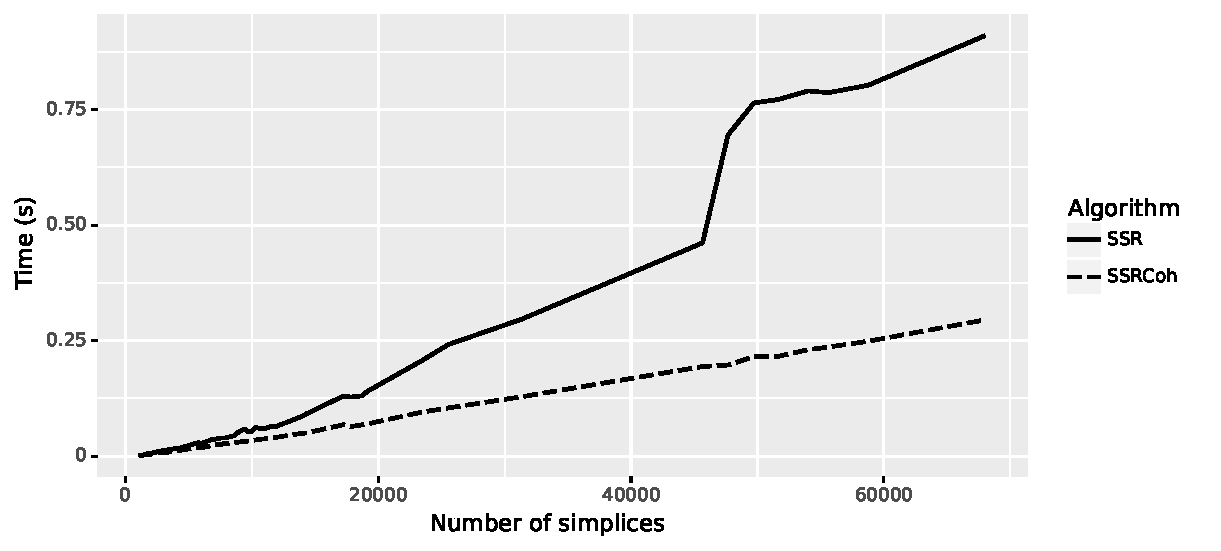
\includegraphics[width=1.2\textwidth]{content/4-comp-top/images/2-3v4-circ-compute}
  }
  \caption{A plot of the running time of \textsc{SSR} and \textsc{SSRCoh} algorithms on a Vietoris-Rips complex constructed from a noisy unit circle.}
  \label{fig:speedsup-3v4}
\end{figure}
